\documentclass[ThesisDJ.tex]{subfiles}

\begin{document}
	Das Projekt zur Evaluation verschiedener Softwarelösungen zur Verbesserung der Kommunikation innerhalb von Teams bzw. Verfahren im Bereich J3 wird zwar im Bereich J3 durchgeführt, hängt aber von keinem der existierenden Projekte, Verfahren oder auch Personen insofern ab, als dass sie direkt als Projektmitarbeiter in das Projekt involviert sind. Somit besteht für die Wahl der Arbeitsweise freie Hand und es ist dem Projektteam überlassen, eine passende Arbeitsweise auszuwählen und in der Folge anzuwenden.\\
	Da der Projektauftrag klar definiert und die zur Verfügung stehende Arbeitszeit durch die Laufzeit stark begrenzt ist, wird weitestgehend traditionell gearbeitet, wobei allerdings Änderungen bzw. weitere notwendige Arbeit nach Bedarf auch nachträglich in die Planung eingebracht werden kann, ohne alle Planungsschritte erneut zu durchlaufen. Einzelne Arbeitsschritte können aber auch agil bearbeitet werden, wenn dies für die Durchführung des Arbeitsschrittes voraussichtlich förderlich ist. Zudem werden einige Werkzeuge, wie beispielswiese ein Kanban-Board, verwendet, welche eher dem agilen Projekmanagement zuzuordnen sind. In diesem Sinne kann die Arbeitsweise in diesem Projekt
	als hybrides Projektmanagement bezeichnet werden
	
  \subsection{Ausgangslage}
  Die HZD nutzt derzeit eine Mischung aus Skype for Business, E-Mails und der Aufgabenverwaltung in Microsoft Azure DevOps zur Kommunikation \cite{microsoft_azure_nodate}. 
  Dabei treten mehrere Herausforderungen auf, die die Effizienz und Übersichtlichkeit der Kommunikation beeinträchtigen:

  \begin{enumerate}
    \item \emph{Mangelnde Abbildung paralleler Projekte}: Mitarbeiterinnen und Mitarbeiter der Abteilung J3 sind häufig in mehreren Projekten gleichzeitig tätig. Die vorhandenen Kommunikationskanäle unterstützen diese Anforderungen nur unzureichend.
    \item \emph{Redundanz im Informationsfluss}: Nachrichten aus Azure DevOps werden zusätzlich per E-Mail an die betroffenen Personen weitergeleitet. Dadurch entsteht eine Dopplung von Informationen, was die Unterscheidung neuer Inhalte von bereits gelesenen erschwert.
    \item \emph{Unübersichtlichkeit durch getrennte Kommunikationswege}: Skype for Business wird primär für schnelle Nachrichten verwendet. Während die schnelle Reaktionszeit geschätzt wird, empfinden viele Mitarbeitende den separaten Kommunikationskanal als unübersichtlich.
  \end{enumerate}

  Neben der textbasierten Kommunikation wird auch Skype for Business für Videokonferenzen verwendet, insbesondere im Homeoffice oder bei 
  der Zusammenarbeit mit externen Stakeholdern. Dabei ergeben sich weitere Probleme:

  \begin{itemize}
    \item Externe Stakeholder haben oft Schwierigkeiten, an Meetings teilzunehmen, da ein Skype-for-Business-Account erforderlich ist.
    \item Meeting-Einladungen müssen per E-Mail verschickt werden; eine Einladung über den Chat ist nicht möglich.
  \end{itemize}

  Auf Basis dieser Beobachtungen und Schilderungen aus der Praxis lassen sich die zu lösenden Probleme wie folgt zusammenfassen:

  \begin{enumerate}
    \item Es gibt zu viele unabhängige Kommunikationswege innerhalb von Projekten
    \item exteren Stakeholder können nicht effizient in die Prozesse eingebunden werden 
    \item Redundante Verbreitung von Informationen, die die Nachverfolgbarkeit erschwert
  \end{enumerate}

	\subsection{Projektbewertung}
  Das Vorhaben zur Lösung der beschriebenen Probleme ist speziell auf die internen Anforderungen und Rahmenbedingungen der HZD abgestimmt 
  und weist einen klar definierten zeitlichen Rahmen auf. Außerdem soll das Vorhaben in einem fixen Personenkreis bearbeitet werden.
  Damit erfüllt es die formelle Definition eines Projekts als ein einmaliges, zeitlich begrenztes und individuelles Vorhaben,
  welches von einem projektspezifisch organisiertem Perosnenkreis bearbeitet wird \cite{bronimann_projektmanagement_2022}. 
  Da das Projekt darauf abzielt, einen bestehenden Prozess zu analysieren und durch konkrete Maßnahmen zu verbessern, 
  handelt es sich um ein typisches Prozessoptimierungsprojekt \cite[S.~8]{kuster_handbuch_2022}. Die Kombination aus Problemanalyse und Umsetzung 
  gezielter Verbesserungen entspricht den Merkmalen dieser Projektkategorie. \\

  Die entstehenden Kosten belaufen sich auf die reinen Personalkosten, da keine spezifischen Mittel oder Infrastruktur benötigt werden. Der entstehende
  Nutzen durch eine reibungslosere Kommunikation könnte eine allgemeine gesteigerte Effizient bei der Umsetzung von Projekten in der Abteilung sein.
	
	\subsection{Ziele}
  Für das Projekt lassen sich zwei Ziele definieren, die für den erfolgreichen Projektabschluss erfüllt sein müssen.
  Zum einen soll ein Maßnahmenkatalog bis zum 17.03.2025 erstellt werden, welche konkrete Empfehlungen zur Verbesserung der Kommunikation
  enthält. Außerdem soll bis zum 31.03.2025 ein Proof-of-Concept mit Dokumentation bereitgestellt werden, welcher eine exemplarische Umsetzung
  der Maßnahmen darstellt. 

  \subsection{Stakeholderanalyse}
  Im folgenden Abschnitt wird eine ausführliche Stakeholderanalyse nach Kuster et al. \cite[S.~86ff]{kuster_handbuch_2022} betrieben, um die sozialen Einflussfaktoren
  auf das Projekt einzuschätzen und im späteren Verlauf ein effektives Stakeholdermanagement durchführen zu können. \\

  Der Auftraggeber ist in diesem Fall ein Stakeholder mit hohem Einfluss und positiver Einstellung. Als Auftraggeber ist er 
  am Erfolg des Projektes interessiert. Er erwartet, dass am Ende die Projektziele erfüllt werden und ein sinnvoller Plan zur Verbesserung 
  der Kommunikation als Endergebnis steht. \\

  Der Bereich J3 ist ein weiterer Stakeholder, welcher für das Projekt von Bedeutung ist. Er ist von den zu treffenden Maßnahmen direkt 
  betroffen, da er die neue Kommunkationsstrategie umsetzen muss. Seine Einstellung ist als neutral zu werten, da er sich zwar eine 
  Ablösung des aktuellen Zustands wünscht, jedoch die neue Lösung von dem Bereich auch akzeptiert werden muss. Es sollten daher aktive 
  Maßnahmen getroffen werden, um sicherzustellen, dass die Akzeptanz für das Projekt und die Ergebnisse hoch bleibt. \\

  Der Leiter der Abteilung J3 kann ebenfalls als Stakeholder gesehen werden, da er ebenfalls Erwartungen an die vorgeschlagenen Lösungen hat.
  Er erhofft sich eine Steigerung und Vereinfachung der Kommunikation im Bereich und daraus auch eine erhöhte Produktivität. Da er für 
  umzusetzende Lösungen sein Einverstängnis geben muss, ist sein Einfluss als sehr hoch anzusehen. Seine Einstellung gegenüber dem Projekt 
  ist als eher neutral zu werten. \\

  Behörden, namentlich die HZD selbst und ihr übergeordnete Behörden wie das Hessische Ministerium für Finanzen oder das Hessische Ministerium 
  für Digitales sind ebenfalls Stakeholder. Durch die Tatsache, dass sie der HZD direkt übergeordnet sind, haben sie einen hohen Einfluss. Dazu 
  ist ihre Einstellung gegenüber dem Projekt als negativ zu bewerten, da organisationsübergreifende Lösungen von ihnen stark bevorzugt werden.
  Im Falle eines möglichen Eingreifens sollte daher vorbereitend geklärt werden, wie man darauf als Projektteam reagiert. \\

  Die Ergebnisse der Stakeholderanalyse sind in \ref{fig:stakeholders} als Matrix aufgelistet.

  \subsection{Stakeholder}
    \begin{figure}[h!]
      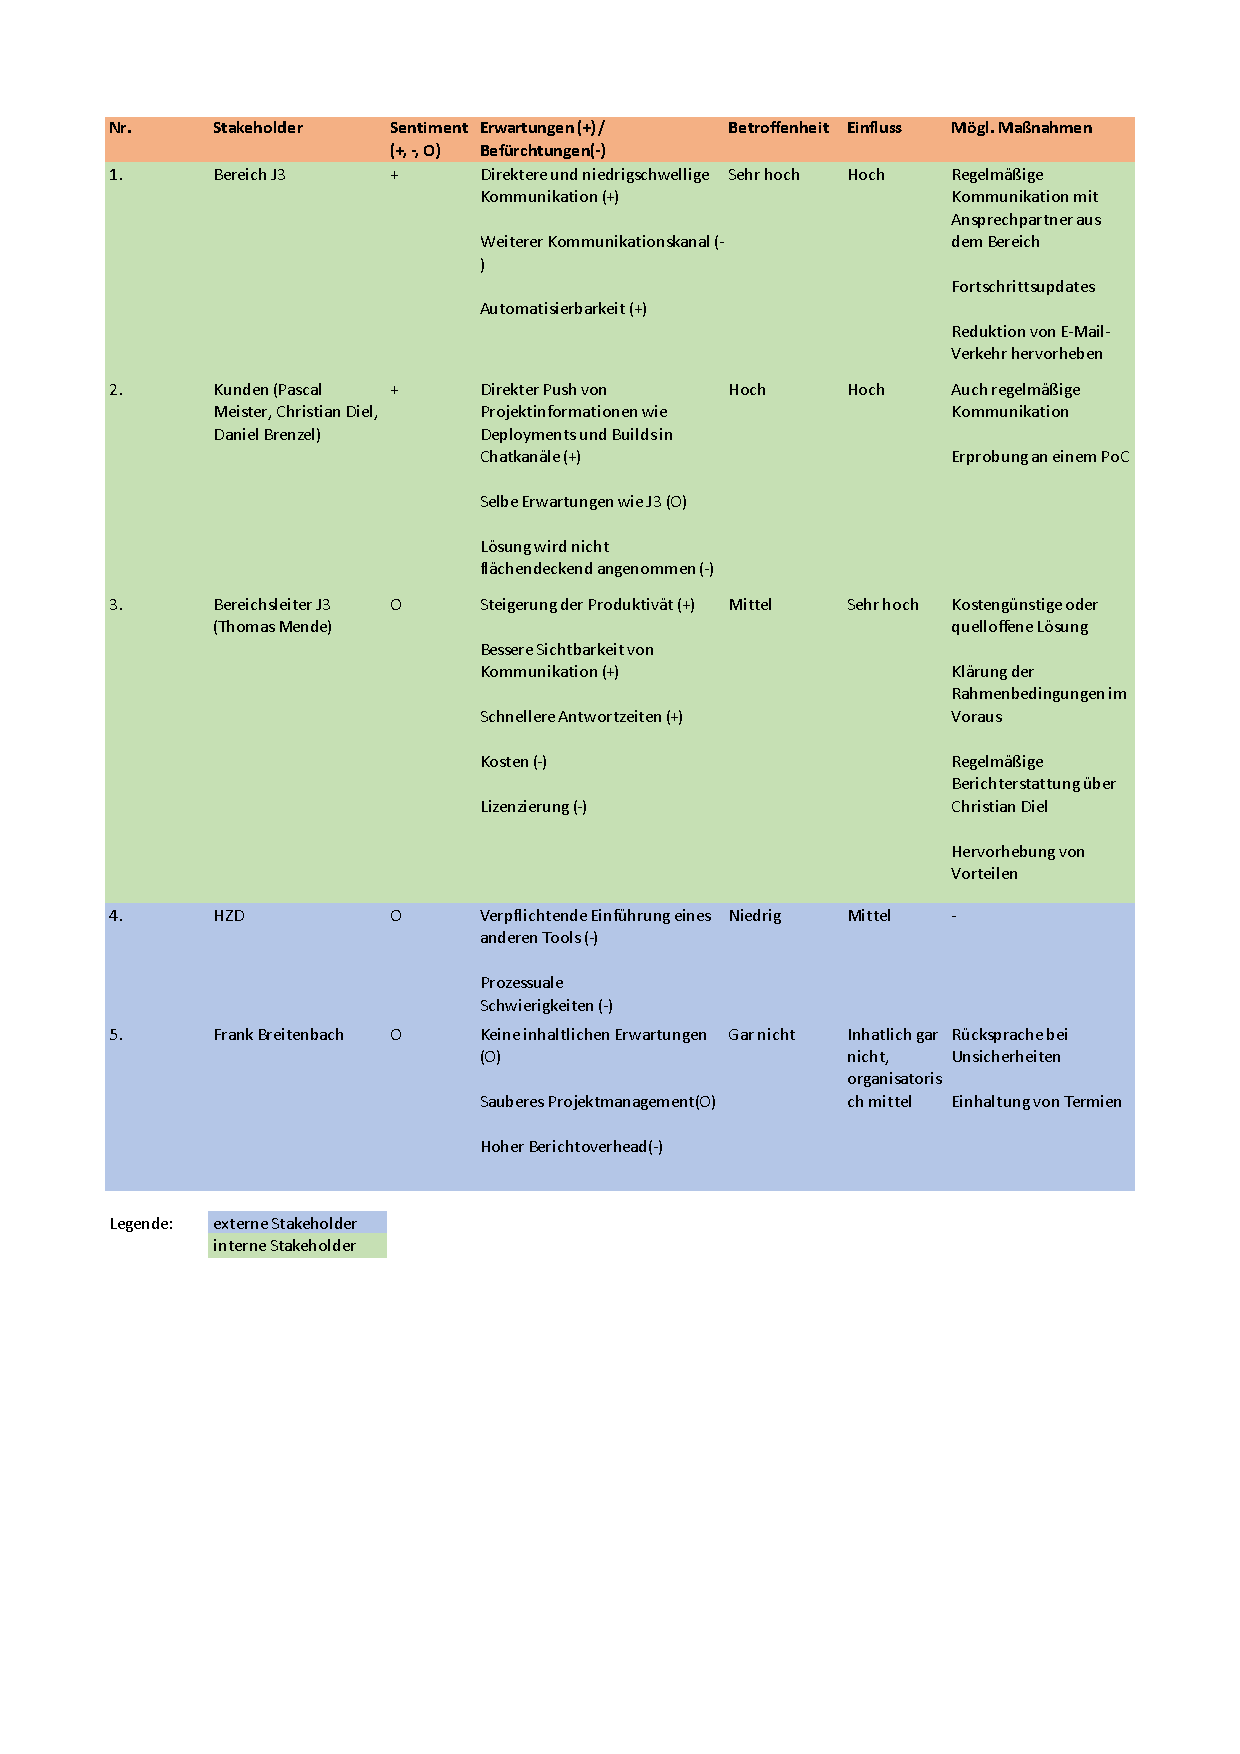
\includegraphics[width=\textwidth]{Stakeholdermatrix.pdf}
      \centering
      \caption{Stakeholdermatrix des Projekts}
      \label{fig:stakeholders}
    \end{figure}

	
	\subsection{Projektauftrag}
	
	Der Projektauftrag gliedert sich in mehrere Punkte, die im Folgenden beschrieben sind:\bigskip\\
	\textbf{Zielsetzung:}\medskip\\
	Wie bereits im Kapitel zu den Zielen ausführlich beschrieben, bestehen zwei Ziele für das Projekt. Nach einer Evaluation verschiedener Softwarelösungen, die eine Empfehlung für eine der evaluierten Lösungen zum Ziel hat, soll als zweites Ziel die Software, für die eine Empfehlung ausgesprochen wurde ein Proof of Concept aufgesetzt werden, zu dem eine Konfigurationsanleitung für den praktischen Einsatz erstellt wird, die dann vom Bereich J3 verwendet werden kann.\bigskip\\
	\textbf{Vorgehensplan:}\medskip\\
	Als Vorgehensplan wurden initial Meilensteine aufgestellt und mit Terminen versehen, zu denen sie abgeschlossen sein sollten. Diese Meilensteine sowie weitere Details zur Zeitplanung werden im entsprechenden Kapitel näher erläutert.\bigskip\\
	\textbf{Abhängigkeiten und Einflussgrößen:}	\medskip\\
	Wie in der Stakeholdermatrix (Link zu Bild/Kapitel) zu sehen ist, existieren verschiedene Stakeholder, die allerdings alle innerhalb der HZD zu verorten sind. Da es sich beim beschriebenen Projekt um ein Projekt innerhalb des Bereichs J3 handelt, dessen Resultat primär auch nur in diesem Bereich eingesetzt werden soll, werden alle Stakeholder, die außerhalb des Bereichs J3 angesiedelt sind, als externe Stakeholder betrachtet. Dies ermöglicht eine genauere Differenzierung der verschiedenen Stakeholder innerhalb der HZD.\bigskip\\
	\textbf{Personalressourcen und Projektorganisation:}\medskip\\
	Für das Projekt stehen 3 Duale Studenten der HZD im Bereich J3 im Projektzeitraum jeweils einen Tag in der Woche zur Verfügung, es kann also mit 3 Personentagen pro Woche für den gesamten Projektzeitraum gerechnet werden, in der Summe sind das 45 Personentage.
	Aufgrund der sehr kleinen Teamgröße gibt es keinen festen Projektleiter, das Vorgehen und die Aufgabenverteilung werden in gemeinsamen Besprechungen festgelegt und miteinander abgestimmt.\bigskip\\
	\textbf{Schätzung der Projektkosten:}\medskip\\
	Die Projektkosten selbst beschränken sich weitestgehend auf die Personalkosten der Projektmitarbeiter.
	Es muss für das Projekt keine zusätzliche Hardware angeschafft werden, an Kosten für Software fällt gegebenenfalls die Lizenzgebühr für die im Proof of Concept zu betrachtende Software an.\bigskip\\
	\textbf{Rahmenbedingungen und Risiko:}\medskip\\
	Wie bei den Personalressourcen bereits beschrieben ist ein wichtiger Faktor im Projekt die geringe wöchentliche Arbeitszeit am Projekt aller Teammitglieder von einem Arbeitstag pro Woche.\\	
	In der HZD wird aktuell ein Wechsel von Skype zu Webex als Kommunikationsplattform erwogen. Wenn dieser Wechsel erfolgt, könnte die Nutzung einer zusätzlichen Softwarelösung obsolet werden, da mit Webex ein Teil der von der Softwarelösung geforderten Funktionen bereits abdeckt werden und sich der Aufwand, für die verbleibenden Funktionen eine zusätzliche Software zu verwenden gegebenenfalls nicht lohnt. Somit ist ein Wechsel zu Webex ein Projektrisiko, da dadurch das Projektergebnis nutzlos werden könnte. 

	
	\subsection{Dokumentationsform}
	
	Die Lieferobjekte des Projekts bestehen, wie im Projekt-Canvas ebenfalls zu sehen sein wird, aus einer Entscheidung für ein einzusetzendes Programm, das den Zweck der verbesserten Kommunikation erfüllt, zusammen mit einer Dokumentation des Evaluationsprozesses sowie einem Proof of Concept zur Konfiguration der ausgewählten Software.\\
	Dementsprechend wird die Dokumentation ebenfalls zweigeteilt sein. Der erste Teil wird abgedeckt durch die Dokumentation des Evaluationsprozesses, die Teil des Lieferobjektes ist, im zweiten Teil wird der Proof of Concept dokumentiert in Form einer Wiki, die die Nutzung und insbesondere die Konfiguration des gewählten Programms beschreibt. 
	
	\subsection{Projekt-Canvas}
  \begin{figure}
    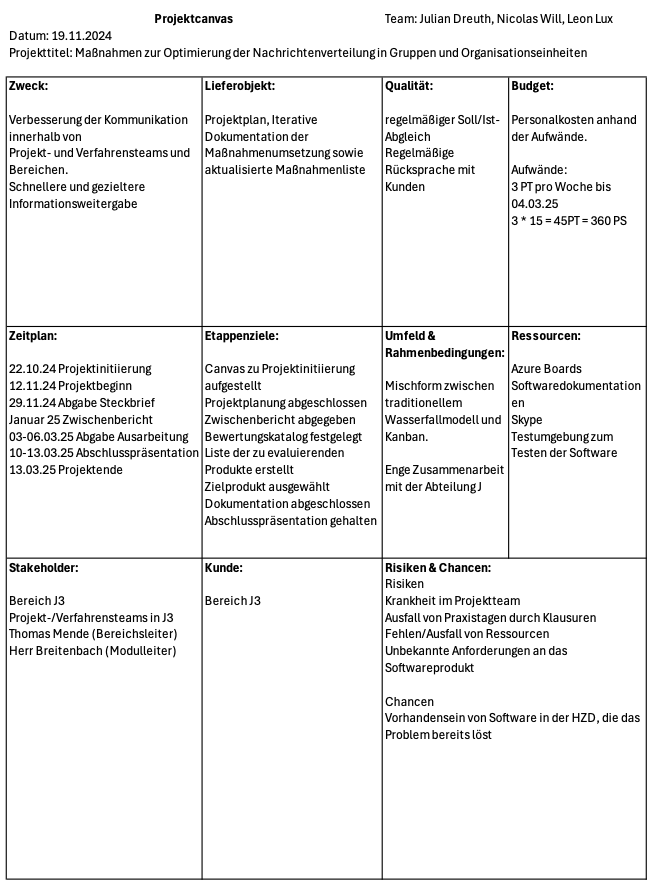
\includegraphics[scale=0.5]{Projektcanvas.png}
    \centering
    \caption{Projektcanvas}
  \end{figure}
\end{document}
